\documentclass[11pt]{article}

\usepackage{amsmath,amssymb}
\usepackage{graphicx}
\usepackage[hyphens]{url}
\usepackage{hyperref}
\usepackage{booktabs}
\usepackage{longtable}
\usepackage{array}
\usepackage{tikz}
\usetikzlibrary{arrows.meta,positioning}

\emergencystretch=3em

% Breakable monospace path (allows line breaks at / and _)
\newcommand{\lpath}[1]{\texttt{\nolinkurl{#1}}}

% Breakable monospace identifier (allows line breaks at _)
\newcommand{\lid}[1]{{\ttfamily\nolinkurl{#1}}}
\newcolumntype{L}[1]{>{\raggedright\arraybackslash}p{#1}}

\title{PLN as a Common Substrate for Naive Bayes and k-NN Premise Selection}
\author{Mettapedia Working Notes}
\date{\today}

\begin{document}
\maketitle

\begin{abstract}
We present an evidence-primary premise-selection calculus in PLN style:
revision (\(\oplus\)) for evidence accumulation, tensor (\(\otimes\)) for
sequential update, and explicit normalization for evidence-budget control.
Classical selectors are represented as specializations on this same carrier:
NB as tensorized likelihood evidence (formal bridge in Lean), and k-NN as
local evidence aggregation (formal bridge to MaSh-style relevance).
We state all log-odds/pooling claims under explicit domain hypotheses:
finite nonzero channels for odds/log-odds theorems, and nonzero finite totals for
normalization/convex-mixture theorems. We also use the corrected pooling result:
hplus is unique under external Bayesianity \emph{plus} total-additivity, with
\lid{max} as the explicit counterexample when total-additivity is omitted.
On extended MPTP 5k validation, round-2 (E, 5s, no \texttt{-p}) yields
290/800 for MaSh NB and 288/800 for the strongest PLN model
(mixture-local Prior\(\otimes\)NB). Round-4 (E+Vampire, 28 runs) has
mixture-local as the best single route on E (288/800) and best/tied-best on
Vampire (174/800 at top-256, 173/800 at top-512). In targeted 30s top-256
follow-up, MaSh NB and mixture-local tie on E (327/800), with a small Vampire
gap (184/800 vs 182/800).
\end{abstract}

\section{Scope and Commitments}
This paper addresses one concrete question: \emph{which PLN rules are actually
used in our premise selectors, how they compose, and under what formal
hypotheses the key equivalences hold.}

There are two code layers:
\begin{itemize}
\item \textbf{Rule layer}: \lpath{hyperon/PeTTa/lib/lib_pln_xi.metta}
      (xiPLN wrappers over the nuPLN evidence algebra, plus calibrated aliases).
\item \textbf{Selector layer}: PeTTa selectors in
      \lpath{hyperon/PeTTa/demos/pln_*_selector*.metta} and one
      pure-Python selector \lpath{atps/scripts/select_pln_mixture_local_nb.py}.
\end{itemize}

\noindent
Methodologically, we stay in the Goertzel/Nil evidence-first discipline:
the evidence object is primary, probabilities are projections, and composition is
governed by algebraic laws rather than post-hoc score blending.

\section{xiPLN Rule Kernel (lib\_pln\_xi)}
For discrete evidence, xiPLN uses the same carrier as nuPLN:
\[
E=(n^+,n^-),\quad E_1\oplus E_2=(n_1^+ + n_2^+,\, n_1^- + n_2^-),
\]
\[
E_1\otimes E_2=(n_1^+ n_2^+,\, n_1^- n_2^-),\quad
\mathrm{power}(E,w)=(n^{+\,w},n^{-\,w}).
\]
Interpretation used throughout this paper: \(E\) is an unnormalized two-channel
measure over \(\{+,-\}\). Revision (\(\oplus\)) adds evidence mass, tensor
(\(\otimes\)) multiplies channel-wise update factors, and strength/confidence are
projections for ranking and reliability.

Operational views:
\[
\mathrm{strength}(E)=\frac{n^+}{n^+ + n^-},\qquad
\mathrm{confidence}(E;\kappa)=\frac{n^+ + n^-}{n^+ + n^- + \kappa}.
\]
\paragraph{Why include \texorpdfstring{\lid{power}}{power}?}
In this work, \(\mathrm{power}(E,w)\) is used as an explicit
\emph{regraduation/calibration} operator in evidence space
(for IDF, \(\tau\)-gates, and prior/likelihood weighting),
implemented in \lpath{hyperon/PeTTa/pln_inference/pln_evidence.metta}.
It is forwarded unchanged by \lid{nuPLN.power} and
\lid{xiPLN.discrete.power}. This is not a legacy
\lid{Truth_*} rule from \lpath{lib_pln.metta}; it is a calibrated extension
layer over the same \(E=(n^+,n^-)\) carrier.
Its mathematical role is justified by Lean theorems
\lid{Evidence.toOdds_power_rpow} and \lid{Evidence.toLogOdds_power_mul}
(\lpath{Mettapedia/Logic/EvidenceQuantale.lean}):
\[
\log\mathrm{odds}(\mathrm{power}(E,w)) = w\cdot \log\mathrm{odds}(E).
\]
So \(w\) scales evidential impact linearly in log-odds space while keeping all
composition in the evidence algebra (\(\oplus,\otimes\)), rather than as ad-hoc
post-hoc score hacking.
This is continuous with the PLN-book scalar idea (scale evidence mass while
preserving the underlying evidential meaning), but different in mechanism:
book-style scalar acts on total-count weight (the \((s,N)\) view), whereas
\(\mathrm{power}\) acts directly on the \((n^+,n^-)\) carrier to produce linear
log-odds regraduation.

\begin{table}[h]
\centering
\begin{scriptsize}
\begin{tabular}{@{}L{0.44\linewidth}L{0.50\linewidth}@{}}
\toprule
\textbf{Rule name (\lid{lib_pln_xi.metta})} & \textbf{Definition / role} \\
\midrule
\lid{ContextualPriorRevision}
& STV-level revision of global and local prior (\(\oplus\)). \\
\lid{PriorLikelihoodTensorSTV}
& Tensor-compose prior and likelihood evidence, then project to STV. \\
\lid{NormalizedPriorLikelihoodTensor}
& Regrade prior/likelihood via \lid{power}, then tensor-compose and project. \\
\lid{WeakNegativeSafeUpdate}
& Add weak negative evidence by revision: \(E \mapsto E \oplus (0,\epsilon)\). \\
\lid{RegraduatedEvidence}
& Explicit evidence regraduation alias: \(E \mapsto \mathrm{power}(E,w)\). \\
\lid{TensorStrengthEqNBPosterior}
& STV wrapper exposing the NB bridge at the rule API boundary. \\
\bottomrule
\end{tabular}
\end{scriptsize}
\caption{xiPLN rule surface used for selector composition.
All rules are in the \lid{xiPLN.Rule.*} or \lid{xiPLN.Bridge.*} namespace.}
\label{tab:xipln-rules}
\end{table}

\noindent
\textbf{Semantic contract.} xiPLN is an API/calibration facade over nuPLN,
not a new calculus: the discrete carrier and core composition laws are identical
(\(E,\oplus,\otimes\)); xiPLN contributes naming, default calibration parameters,
and task-facing wrappers only.

\begin{table}[h]
\centering
\begin{scriptsize}
\begin{tabular}{p{0.26\linewidth}p{0.67\linewidth}}
\toprule
\textbf{Layer} & \textbf{Provenance / semantic status} \\
\midrule
Legacy PLN rules & \lid{Truth_*} rules in \lpath{hyperon/PeTTa/lib/lib_pln.metta},
with direct PLN-book grounding (e.g., \lid{Truth_Revision}, book \S5.10.2). \\
Evidence-calibration extension & \lid{evidence-hplus}, \lid{evidence-tensor},
\lid{evidence-power} in \lpath{pln_inference/pln_evidence.metta}, wrapped by
\lid{nuPLN}/\lid{xiPLN}; coherence justified by Lean evidence theorems listed in
Section~\ref{sec:leanmap}. \\
\bottomrule
\end{tabular}
\end{scriptsize}
\caption{Legacy-vs-extension provenance for the rules used in this paper.}
\label{tab:legacy-vs-extension}
\end{table}

\subsection{Rule list (precise mathematical form)}
For a goal \(g\), candidate premise \(a\), and evidence values
\(E=(n^+,n^-)\), \(F=(m^+,m^-)\in \mathbb{R}_{\ge 0}^{\infty}\times\mathbb{R}_{\ge 0}^{\infty}\):
\begin{align*}
\textbf{R1 (Revision)}\quad
E \oplus F &:= (n^+ + m^+,\; n^- + m^-),\\
\textbf{R2 (Tensor update)}\quad
E \otimes F &:= (n^+ m^+,\; n^- m^-),\\
\textbf{R3 (Strength projection)}\quad
s(E) &:= \frac{n^+}{n^+ + n^-},\\
\textbf{R4 (Confidence projection)}\quad
c_\kappa(E) &:= \frac{n^+ + n^-}{n^+ + n^- + \kappa},\\
\textbf{R5 (Regraduation)}\quad
\mathrm{pow}_w(E) &:= (n^{+\,w},\; n^{-\,w}),\\
\textbf{R6 (Normalization)}\quad
\mathrm{Norm}_t(E) &:= \big(t\,s(E),\; t(1-s(E))\big),\\
\textbf{R7 (Weak negative safety)}\quad
\mathrm{WeakNeg}_\epsilon(E) &:= E \oplus (0,\epsilon),\\
\textbf{R8 (Staged selector posterior)}\quad
E_{\mathrm{post}}(g,a) &:=
\Big(\bigoplus_i \mathrm{Norm}_{t_i(g)}(\mathrm{pow}_{w_i}(E_i(g,a)))\Big)\\
&\quad\otimes \mathrm{Norm}_{t_L}(E_{\mathrm{like}}(g,a)).
\end{align*}

\noindent
Ranking is then performed by
\(
\mathrm{score}(g,a):=s(E_{\mathrm{post}}(g,a))
\),
with optional confidence-aware tie-breaking via \(c_\kappa\).

\noindent
These are not free-floating definitions: they are tied to Lean contracts listed
in Section~\ref{sec:leanmap}, including log-odds additivity under tensor,
linear log-odds scaling under regraduation, normalization-preserves-strength,
and staged commutation laws.

\begin{table}[h]
\centering
\begin{scriptsize}
\begin{tabular}{@{}L{0.18\linewidth}L{0.35\linewidth}L{0.40\linewidth}@{}}
\toprule
\textbf{Rule} & \textbf{Lean contract} & \textbf{Implementation locus} \\
\midrule
R1 (\(\oplus\), revision) &
\lid{PLN_revisionStrength_eq_linearPool} &
\lpath{pln_inference/pln_evidence.metta}, \lid{xiPLN.Rule.ContextualPriorRevision} \\
R2 (\(\otimes\), update) &
\lid{Evidence.toLogOdds_tensor_add} &
\lpath{pln_inference/pln_evidence.metta}, \lid{xiPLN.Rule.PriorLikelihoodTensorSTV} \\
R5 (\(\mathrm{pow}\), regraduation) &
\lid{Evidence.toLogOdds_power_mul} &
\lpath{pln_inference/pln_evidence.metta}, \lid{xiPLN.Rule.RegraduatedEvidence} \\
R6 (\(\mathrm{Norm}\), mass control) &
\lid{normalizeEvidence_toStrength} &
\lpath{Mettapedia/Logic/PremiseSelectionFusion.lean}, normalized selector stages \\
R8 (staged posterior map) &
\lid{stagedFamilyPosterior_commute},\\
\lid{stagedFamilyPosterior_regrade_roundtrip_commute} &
\lpath{atps/scripts/select_pln_mixture_local_nb.py} \\
\bottomrule
\end{tabular}
\end{scriptsize}
\caption{Compact rule$\rightarrow$theorem$\rightarrow$implementation crosswalk.}
\label{tab:rule-crosswalk}
\end{table}

\subsection{Formal domain assumptions (explicit)}
Claims such as ``log-pool equivalence'' or ``additivity in log-odds'' are
\emph{not} unconditional in our Lean development; they are theorem-level claims
under explicit hypotheses.
\begin{itemize}
\item \textbf{Tensor in odds/log-odds}:
      \lid{Evidence.toOdds_tensor_mul} and
      \lid{Evidence.toLogOdds_tensor_add} require finite/nonzero regime
      assumptions (notably nonzero negative channels and finite/nonzero odds).
\item \textbf{Regraduation in log-odds}:
      \lid{Evidence.toLogOdds_power_mul} requires \(w \ge 0\), \(n^- \neq 0\),
      and finite/nonzero odds.
\item \textbf{Normalization contracts}:
      \lid{normalizeEvidence_toStrength} and
      \lid{fuse_toStrength_normalized_totals} require \(t \neq 0\) and
      \(t \neq \top\) (finite nonzero evidence totals).
\end{itemize}

\noindent
Accordingly, all selector equations in this paper are understood in that same
finite/nonzero regime unless stated otherwise.
When we say ``log-pool'' in this paper, we mean this precise theorem-backed
statement: channel-wise tensor update induces additive log-odds under the
hypotheses of \lid{Evidence.toLogOdds_tensor_add}.

\section{How Rules Are Composed in Our Selectors}
\subsection{IDF-NB selector (likelihood-heavy baseline)}
Files:
\lpath{hyperon/PeTTa/demos/pln_idf_nb_selector_jobs.metta},
\lpath{atps/scripts/select_pln_nb.py}.

Construction:
\begin{itemize}
\item Prior evidence per axiom from tfreq table.
\item Feature evidence from \lid{lookup_feature_idf_db} with IDF weights.
\item Log-domain fold over features:
      \(\log P^+,\log P^-\) accumulated with weighted \(\log n^+,\log n^-\).
\item STV projection:
      \(\mathrm{strength}=\sigma(\log P^+-\log P^-)\),
      confidence from a log-total vs \(\log\kappa\) gate.
\end{itemize}

\subsection{kNN-prior + NB-likelihood (PeTTa merged model)}
Files:
\lpath{hyperon/PeTTa/demos/pln_knn_prior_nb_selector_opt.metta},
\lpath{atps/scripts/select_pln_knn_prior_nb_opt.py}.

Construction:
\begin{itemize}
\item Per-neighbor overlap (\texttt{goal\_feat\_db} $\cap$ \texttt{nbr\_feat\_db})
      computed in Prolog backend.
\item Canonical evidence transfer is kNN-positive / weak-negative aggregation:
      used neighbors contribute \((w,0)\), non-used neighbors contribute
      \((0,\eta w)\), then rows are aggregated by \lid{evidence-hplus}.
\item The legacy PeTTa implementation includes a modus-ponens-style row transfer
      in \lpath{pln_rules.metta}; in this paper, the semantic contract is the
      evidence-level transfer above (which is what the Lean kNN bridge captures).
\item Goal prior is revised:
      \(E_{\text{prior}}=E_{\text{global}} \oplus E_{\text{knn}}\).
\item NB likelihood (features only) is composed in log-domain with
      prior odds to produce final STV.
\end{itemize}

\noindent
\fbox{
\parbox{0.975\linewidth}{
\textbf{Legacy MP vs canonical transfer.}
The PLN book treats probabilistic MP as useful but heuristic/error-prone.
For premise selection we therefore take evidence-level kNN transfer
(\((w,0)\) for used, \((0,\eta w)\) for weak-negative) as canonical semantics,
and treat MP-style row transfer as a legacy implementation detail.
}}

\subsection{Mixture-local Prior\texorpdfstring{$\otimes$}{x}NB (staged model)}
File:
\lpath{atps/scripts/select_pln_mixture_local_nb.py}.

This is the explicit staged architecture:
\begin{itemize}
\item \textbf{Stage A}: build multiple local experts from neighborhood bins
      \([4,16,64,256]\), with weak negatives.
\item \textbf{Stage B}: normalize each expert to target mass and pool via
      evidence addition (\(\oplus\)).
\item \textbf{Stage C}: tensor-compose pooled prior with likelihood-only NB
      evidence (\(\otimes\)).
\end{itemize}
Formally:
\begin{multline*}
  E_{\text{post}}(g,a)=
  \Big(
    \bigoplus_i \mathrm{Normalize}_{t_i(g)}(E_i^{\text{local}}(g,a))
    \oplus \mathrm{Normalize}_{t_G}(E^{\text{global}}(a))
  \Big)\\
  {}\otimes \mathrm{Normalize}_{t_L}(E^{\text{NB-like}}(g,a)).
\end{multline*}
The staged map commutes in the external-Bayes sense and is stable under
regrade/unregrade round-trip:
\lid{stagedFamilyPosterior_commute} and
\lid{stagedFamilyPosterior_regrade_roundtrip_commute}
(\lpath{Mettapedia/Logic/PremiseSelectionExternalBayesianity.lean}).

\begin{figure}[h]
\centering
\resizebox{0.98\linewidth}{!}{
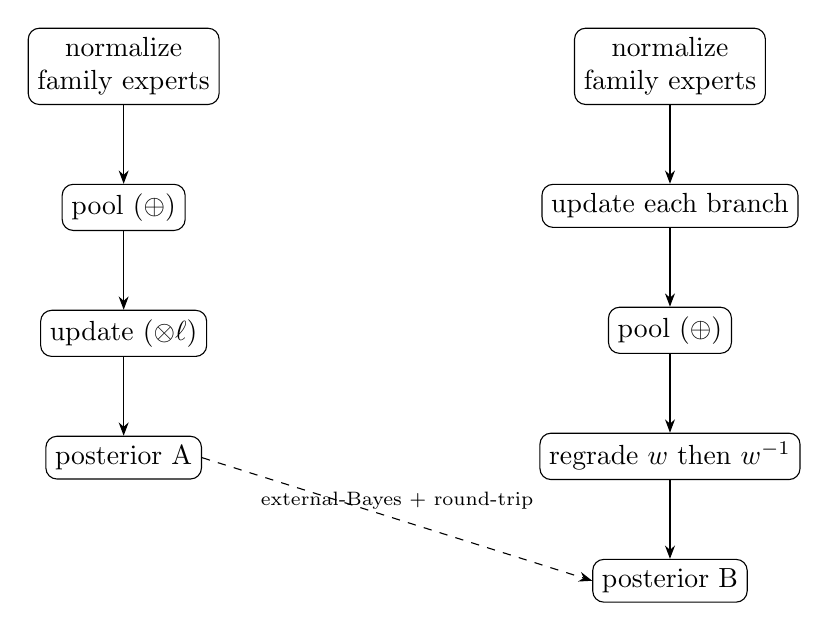
\begin{tikzpicture}[>=Stealth,node distance=10mm and 20mm]
  \node (L0) [draw,rounded corners,align=center] {normalize\\family experts};
  \node (L1) [draw,rounded corners,align=center,below=of L0] {pool ($\oplus$)};
  \node (L2) [draw,rounded corners,align=center,below=of L1] {update ($\otimes \ell$)};
  \node (LP) [draw,rounded corners,align=center,below=of L2] {posterior A};

  \node (R0) [draw,rounded corners,align=center,right=45mm of L0] {normalize\\family experts};
  \node (R1) [draw,rounded corners,align=center,below=of R0] {update each branch};
  \node (R2) [draw,rounded corners,align=center,below=of R1] {pool ($\oplus$)};
  \node (R3) [draw,rounded corners,align=center,below=of R2] {regrade $w$ then $w^{-1}$};
  \node (RP) [draw,rounded corners,align=center,below=of R3] {posterior B};

  \draw[->] (L0) -- (L1);
  \draw[->] (L1) -- (L2);
  \draw[->] (L2) -- (LP);

  \draw[->] (R0) -- (R1);
  \draw[->] (R1) -- (R2);
  \draw[->] (R2) -- (R3);
  \draw[->] (R3) -- (RP);

  \draw[->,dashed] (LP.east) -- node[above] {\scriptsize external-Bayes + round-trip} (RP.west);
\end{tikzpicture}
}
\caption{Commuting staged selector diagram for the normalized family pool/update
pipeline with regrade round-trip coherence.}
\label{fig:staged-commuting}
\end{figure}

\subsection{Unified selector derivation skeleton}
All selectors in this paper instantiate the same calculus template:
\begin{align*}
E^{(i)}_{\text{prior}}(g,a) &\xrightarrow{\ \mathrm{power}\ }\widetilde{E}^{(i)}_{\text{prior}}(g,a)
\xrightarrow{\ \mathrm{Normalize}_{t_i(g)}\ }\widehat{E}^{(i)}_{\text{prior}}(g,a), \\
E_{\text{pool}}(g,a) &= \bigoplus_i \widehat{E}^{(i)}_{\text{prior}}(g,a), \\
E_{\text{post}}(g,a) &= E_{\text{pool}}(g,a)\otimes
\mathrm{Normalize}_{t_L}\!\left(E_{\text{like}}(g,a)\right), \\
\mathrm{score}(g,a) &= \mathrm{strength}\!\left(E_{\text{post}}(g,a)\right).
\end{align*}
NB-only, kNN+NB, and mixture-local models differ only in how
\(E^{(i)}_{\text{prior}}\), \(t_i\), and \(E_{\text{like}}\) are instantiated.
The operator laws are shared.

\section{Lean Contracts for the Rule Stack}
The implementation-level rules above are tied to explicit Lean contracts.
Abbreviation: \texttt{EB} = \lpath{PremiseSelectionExternalBayesianity.lean}.

\paragraph{Core bridges.}
\begin{itemize}
\item \textbf{NB bridge}: \lid{toStrength_nbEvidence_eq_nbPosterior}\\
      (\lpath{PLNBayesNetInference.lean}).
\item \textbf{k-NN bridge}: \lid{PLN_hplusPos_eq_knnRelevance}\\
      (\lpath{PremiseSelectionKNN_PLNBridge.lean}).
\item \textbf{Revision = linear pooling}:\\
      \lid{PLN_revisionStrength_eq_linearPool}
      (\lpath{PremiseSelectionFusion.lean}).
\item \textbf{Prior/NB two-stage}:\\
      \lid{priorNBPosterior_eq_twoStage}
      (\lpath{PremiseSelectionPriorNB.lean}).
\end{itemize}

\paragraph{Evidence-algebra laws (in \lpath{EvidenceQuantale.lean}).}
Regraduation: \lid{Evidence.toLogOdds_power_mul},
\lid{Evidence.toOdds_power_rpow}.
Round-trip canaries: \lid{Evidence.power_power_inv},
\lid{Evidence.toLogOdds_power_power_inv}.

\paragraph{Normalization and fusion (in \lpath{PremiseSelectionFusion.lean}).}
\lid{normalizeEvidence_toStrength} (preserves strength for $t\neq 0$, $t\neq\top$);
\lid{fuse_toStrength_normalized_totals} (explicit convex weights).

\paragraph{Pooling uniqueness (in \texttt{EB}).}
\lid{poolE_eq_hplus_of_externalBayes_totalAdd} (hplus is unique under
external Bayesianity + total-additivity),
plus counterexample \lid{maxPoolingOperator_ne_fuse}.

\paragraph{Regrading and staged coherence (in \texttt{EB}).}
\lid{toLogOdds_scaleEvidence} (regrading invariance);
\lid{externalBayesianity_fuseFamily_tensor} (family-level commutation);
\lid{stagedFamilyPosterior_commute} and
\lid{stagedFamilyPosterior_regrade_roundtrip_commute} (staged-pipeline canaries).

\paragraph{Additional contracts.}
\lid{finite_statistic_tv_mixture_bound_m16_R4551}
(\lpath{PremiseSelectionLocalMixtureBridge.lean});
\lid{fusion_ranking_after_normalization_toReal}
(\lpath{PremiseSelectionOptimality.lean});
OSLF modal corollaries \lid{oslf_diamond_stagedFamily_roundtrip} and
\lid{oslf_box_stagedFamily_roundtrip}
(\lpath{OSLF/Framework/PLNSelectorGSLT.lean}).

\noindent
For a selector-level composition theorem that mirrors the staged architecture, see
\lpath{Mettapedia/Logic/PremiseSelectionBestPLNDraft.lean}.

\section{Experimental validation on extended MPTP 5k (rounds 1--4)}
\subsection{Protocol and data integrity}
We evaluate seven selectors under one canonical protocol:
\begin{itemize}
\item Dataset: 4200 train problems, 800 validation problems.
\item Model-generation data source: pooled dependency events\footnote{In
      evidential semantics, a ``round'' is a data-provenance epoch (new proof
      observations), not a new logical calculus. Pooling rounds means accumulating
      additional evidence counts via revision (\(\oplus\)); normalization keeps
      evidence budgets explicit before tensor composition (\(\otimes\)).
      Thus round labels record chronology/integrity of evidence acquisition, while
      core PLN operators remain fixed.}
      (\lpath{pooled_train_deps_allruns.jsonl}), built from base train deps
      plus prior train proof runs; final pool size is 9045 events over 1649 unique
      training problems.
\item Selection budgets: top-256 and top-512.
\item Prover route: E 3.0.1-ho, timeout 5s, jobs=4, \emph{without} E's \texttt{-p}.
\item Integrity policy: generate top-512 selections first, derive top-256 by prefix
      truncation, then run E on both budgets.
\end{itemize}

\noindent
We report: (i) round-1 reference validation, (ii) round-2 pooled-data
validation, and (iii) round-4 cross-prover validation.
Training \emph{rounds} refer to provenance epochs for building pooled training
evidence, while validation \emph{runs} are fixed-budget prover executions on the
held-out 800-problem split using selectors trained from that pooled evidence.

\subsection{Methods in PLN rule style}
In the PLN book spirit, we keep evidence as the primary object and use only:
revision (\(\oplus\), evidence accumulation), tensor (\(\otimes\), sequential
composition), and normalization (fix evidence mass while preserving strength).
Across training rounds, we accumulate dependency evidence by revision:
\[
  E_{\mathrm{pool}}(a)=\bigoplus_{r\in\mathcal{R}} E_r(a),
\]
where \(E_r(a)\) is the evidence contribution for premise \(a\) from round \(r\).
Thus, adding rounds means adding evidence mass in the same algebra; it does not
change the selector logic or operator semantics.

For the new mixture-local selector (\lpath{select_pln_mixture_local_nb.py}),
the staged construction is:
\begin{multline*}
  E_{\text{post}}(g,a) =
  \Big(
    \bigoplus_i \mathrm{Normalize}_{t_i(g)}(E_i^{\text{local}}(g,a))
    \oplus \mathrm{Normalize}_{t_G}(E^{\text{global}}(a))
  \Big)\\
  {}\otimes
  \mathrm{Normalize}_{t_L}(E^{\text{NB-like}}(g,a)).
\end{multline*}
Here each local expert \(i\) is built from a k-NN bin:
\[
  n_i^+(g,a)=\sum_{\chi\in B_i(g)} \mathrm{sim}(g,\chi)\,\mathbf{1}[a\in deps(\chi)],
\]
\[
  n_i^-(g,a)=\eta\sum_{\chi\in B_i(g)} \mathrm{sim}(g,\chi)\,\mathbf{1}[a\notin deps(\chi)].
\]
We use \(E_i^{\text{local}}=(n_i^++\alpha,\;n_i^-+\beta)\), with weak-negative
factor \(\eta=0.08\), bins \([4,16,64,256]\), and similarity
\(\mathrm{sim}=\mathrm{overlap}/(\mathrm{overlap}+\kappa)\).
Likelihood evidence is \emph{NB-likelihood only} (prior removed by setting
\(\sigma_1=0\)), then robustly scaled per problem (IQR target) before conversion
to odds evidence and normalization.

This gives a non-alias architecture:
\begin{itemize}
\item Stage A: multiple local priors from neighbor bins.
\item Stage B: normalized pooling via revision (\(\oplus\)).
\item Stage C: normalized tensor with likelihood-only NB evidence.
\end{itemize}

\noindent
\textbf{What this claims (and does not).}
The Lean contracts certify algebraic coherence of the selector pipeline
(pool/update/regrade/normalize laws under stated hypotheses). They do not prove
that any one concrete script is globally optimal for ATP success under fixed
time budgets. Empirical quality still depends on data quality, feature design,
and calibration of local evidence reliability.

\subsection{Round-1 reference results}
To keep the chronology explicit, Table~\ref{tab:r1val} lists the pre-pooled
round-1 validation runs used before the round-2 pooled-data refresh.

\begin{table}[h]
\centering
\begin{scriptsize}
\begin{tabular}{p{0.44\linewidth}rr}
\hline
Model (round1 reference) & Top-256 & Top-512 \\
\hline
MaSh NB & 283/800 (35.38\%) & 291/800 (36.38\%) \\
PLN kNN-prior-NB (opt, merge-NB) & 282/800 (35.25\%) & 291/800 (36.38\%) \\
PLN NB & 281/800 (35.12\%) & n/a \\
PLN Normal-NB & 279/800 (34.88\%) & n/a \\
PLN Enhanced & 276/800 (34.50\%) & n/a \\
MaSh k-NN & 272/800 (34.00\%) & 291/800 (36.38\%) \\
\hline
\end{tabular}
\end{scriptsize}
\caption{Round-1 validation reference results (legacy pre-pooled run set).}
\label{tab:r1val}
\end{table}

\subsection{Validation results (canonical 14 runs)}
Table~\ref{tab:r2val} reports all seven models at top-256 and top-512.

\begin{table}[h]
\centering
\begin{scriptsize}
\begin{tabular}{p{0.44\linewidth}rr}
\hline
Model (round2\_pooled) & Top-256 & Top-512 \\
\hline
MaSh NB & 290/800 (36.25\%) & 285/800 (35.63\%) \\
PLN mixture-local Prior$\otimes$NB & 288/800 (36.00\%) & 286/800 (35.75\%) \\
PLN kNN-prior-NB (opt, merge-NB) & 281/800 (35.12\%) & 285/800 (35.63\%) \\
MaSh k-NN & 280/800 (35.00\%) & 286/800 (35.75\%) \\
PLN Normal-NB & 280/800 (35.00\%) & 282/800 (35.25\%) \\
PLN NB & 276/800 (34.50\%) & 285/800 (35.63\%) \\
PLN Enhanced & 272/800 (34.00\%) & 283/800 (35.38\%) \\
\hline
\end{tabular}
\end{scriptsize}
\caption{Round-2 validation results (E5s, no-\texttt{-p}, jobs=4).}
\label{tab:r2val}
\end{table}

\subsection{Round-2 discussion}
\begin{itemize}
\item \textbf{Top-256 precision regime}: MaSh NB is best (290), but the new
      PLN mixture-local model is very close (288). The margin is 2/800.

\item \textbf{Top-512 recall regime}: MaSh k-NN and PLN mixture-local tie for best
      (286), with MaSh NB and two PLN variants at 285. At this budget, differences
      are effectively tie-level.

\item \textbf{Overlap is high}: at top-256, MaSh NB and PLN mixture-local share
      287 solved problems, with only 3 NB-unique and 1 mixture-unique. At top-512,
      MaSh NB vs MaSh k-NN differs on just 5 problems total.

\item \textbf{Greedy-cover complementarity remains small but real}: top-5 greedy
      union is 297 solved with all runs, and 296 without MaSh runs. So MaSh adds
      one extra unique solve in this top-5 cover view.

\item \textbf{PLN interpretation}: these results match the formal story. Revision
      and tensor composition are structurally correct, but empirical gains depend on
      calibration quality of local priors and gating, not on operator choice.
\end{itemize}

\subsection{Round-4 cross-prover validation (canonical 28 runs)}
Round-4 evaluates seven selector tags across two prover routes (E no-\texttt{-p}
and Vampire), each at top-256 and top-512:
\[
  7 \times 2 \times 2 = 28 \text{ runs}.
\]
Protocol: validation split (800 problems), timeout 5s, jobs=6 for both provers.
The compact artifact is therefore named
\lpath{results_round4_val_5s_compact_28runs.csv}. Separate targeted
top-256 30s runs were executed later for the two strongest models only.

\begin{table}[h]
\centering
\begin{small}
\begin{tabular}{p{0.40\linewidth}rrrr}
\hline
Model (round4 tags) & E@256 & E@512 & V@256 & V@512 \\
\hline
MaSh NB (E-trained) & 284 & 277 & 171 & 172 \\
MaSh NB (V-trained) & 281 & 280 & 170 & 169 \\
MaSh k-NN (E-trained) & 278 & 285 & 171 & 171 \\
MaSh k-NN (V-trained) & 277 & 283 & 170 & 170 \\
PLN kNN-prior-NB+MaSh (E-trained) & 276 & 280 & 170 & 173 \\
PLN kNN-prior-NB+MaSh (V-trained) & 280 & 280 & 172 & 173 \\
PLN mixture-local Prior$\otimes$NB (EV-pooled) & \textbf{288} & \textbf{288} & \textbf{174} & \textbf{173} \\
\hline
\end{tabular}
\end{small}
\caption{Round-4 validation results (E no-\texttt{-p} and Vampire, 5s, jobs=6).}
\label{tab:r4val}
\end{table}

\subsection{Round-4 discussion}
\begin{itemize}
\item \textbf{Best single run}: PLN mixture-local Prior$\otimes$NB is strongest on E
      (288/800) and also best on Vampire at top-256 (174/800), tying best at
      top-512 Vampire (173/800).
\item \textbf{Top-256 vs top-512 behavior}: for the winning model, E@256 and E@512
      are identical (288), indicating ranking saturation by 256 for this setup.
\item \textbf{Vampire spread is compressed}: all Vampire runs lie in a narrow band
      (169--174 solved), suggesting lower sensitivity to selector differences at 5s.
\item \textbf{Cross-route complementarity is real}: greedy cover over all 28 runs
      reaches 321/800, while the top-5 greedy picks already reach 320/800.
\item \textbf{MaSh contribution in cover space}: greedy cover without MaSh-tagged
      runs is 315/800; including MaSh raises the full cover to 321/800.
\end{itemize}

\subsection{Targeted 30s follow-up (top-256)}
To test whether 5s outcomes were dominated by prover-time limits, we ran a
targeted 30s follow-up on the two strongest models from round-4:
MaSh NB (E-trained) and PLN mixture-local Prior$\otimes$NB (EV-pooled), both at
top-256 on the same 800 validation problems.

\begin{table}[h]
\centering
\begin{small}
\begin{tabular}{p{0.44\linewidth}rr}
\toprule
Model (top-256, 30s) & E no-\texttt{-p} & Vampire \\
\midrule
MaSh NB (round4\_e) & 327/800 (40.88\%) & \textbf{184/800} (23.00\%) \\
PLN mixt.-local Prior$\otimes$NB (round4\_ev) & 327/800 (40.88\%) & 182/800 (22.75\%) \\
\bottomrule
\end{tabular}
\end{small}
\caption{Targeted 30s validation follow-up at top-256.}
\label{tab:r4val30}
\end{table}

Interpretation: at longer E time budgets, both models converge to the same solve
count, while on Vampire the gap remains small (2 problems).

\subsection{Implementation notes}
\begin{itemize}
\item ATP drivers:
      \lpath{atps/scripts/select_pln_nb.py},
      \lpath{atps/scripts/select_pln_normal_nb.py},
      \lpath{atps/scripts/select_pln_enhanced.py},
      \lpath{atps/scripts/select_pln_knn_prior_nb_opt.py}.
\item PeTTa selector backends:
      \lpath{hyperon/PeTTa/demos/pln_*_selector*.metta}.
\item Library usage:
      \lpath{hyperon/PeTTa/lib/lib_pln_nu.metta} and
      \lpath{hyperon/PeTTa/pln_inference/pln_evidence.metta}/
      \lpath{hyperon/PeTTa/pln_inference/pln_rules.metta} are the main paths for
      current discrete selectors; \lpath{hyperon/PeTTa/lib/lib_pln_xi.metta}
      is used explicitly in the normal-carrier path and as the rule-level API
      target for the xiPLN exposition in this paper.
\item Pure-Python selector:
      \lpath{atps/scripts/select_pln_mixture_local_nb.py}
      (same evidence algebra, staged explicitly for auditability/performance).
\item Round-4 queue/orchestration:
      \lpath{atps/scripts/run_round4_val_execute_and_analyze.sh}.
\item Round-4 compact scoreboard and greedy artifacts:
      \lpath{results_round4_val_5s_compact_28runs.csv},
      \lpath{greedy_cover_round4_val_all.csv},
      \lpath{greedy_cover_round4_val_no_mash.csv}.
\end{itemize}

\section{Lean map}
\label{sec:leanmap}

All paths are relative to the project root.
Abbreviation: \texttt{M/L/} = \texttt{Mettapedia/Logic/}.

\begin{scriptsize}
\begin{longtable}{@{}L{0.48\linewidth}L{0.48\linewidth}@{}}
\toprule
\textbf{Module} & \textbf{Contents} \\
\midrule
\endhead
\lpath{M/L/EvidenceQuantale.lean}
  & Evidence carrier, semiring/quantale laws, odds/log-odds and power laws \\
\lpath{M/L/PLNCore.lean}
  & Curated top-level import surface for the theorem-complete PLN stack \\
\lpath{M/L/PremiseSelectionKNN.lean}
  & General k-NN definitions; MaSh instance \\
\lpath{M/L/PremiseSelectionKNN_PLNBridge.lean}
  & PLN--k-NN bridge; paper-form equivalence \\
\lpath{M/L/PLNBayesNetInference.lean}
  & PLN NB bridge; strength = NB posterior \\
\lpath{M/L/PremiseSelectionFusion.lean}
  & Fusion via revision; normalization \\
\lpath{M/L/PremiseSelectionOptimality.lean}
  & Optimality transfer lemmas (NB, k-NN, PLN, fusion, ranking) \\
\lpath{M/L/PremiseSelectionExternalBayesianity.lean}
  & Counterexample + corrected uniqueness; regraduation invariance;
    staged commutation canaries \\
\lpath{M/L/PremiseSelectionOperatorRoles.lean}
  & Role discipline structures \\
\lpath{M/L/PremiseSelectionPriorNB.lean}
  & Prior-NB composition; canonical aliases \\
\lpath{M/L/PremiseSelectionLocalMixtureBridge.lean}
  & Finite local-mixture TV bounds \\
\lpath{M/L/DiaconisFreedmanFinite.lean}
  & Base collision bound \\
\lpath{M/L/PremiseSelectionCoverage.lean}
  & Submodular coverage \\
\lpath{M/L/PremiseSelectionPUCalibration.lean}
  & PU weak-negative calibration \\
\lpath{M/L/PremiseSelectionRankingStability.lean}
  & Ranking stability \\
\lpath{M/L/PremiseSelectionSelectorSpec.lean}
  & Selector spec defaults/checklist \\
\lpath{M/L/PremiseSelectionPartitionedPriorNB.lean}
  & Partitioned normalized Prior-NB \\
\lpath{hyperon/PeTTa/tests/test_lib_pln_xi_rules.metta}
  & Deterministic xiPLN rule tests \\
\bottomrule
\end{longtable}
\end{scriptsize}

\end{document}
